\begin{center}
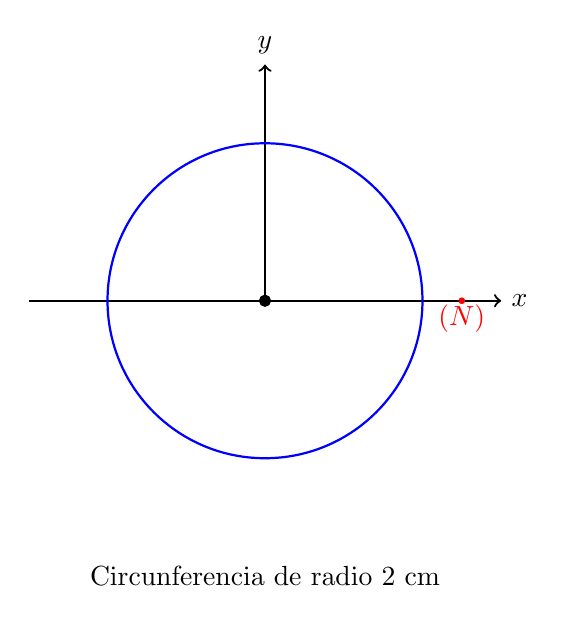
\begin{tikzpicture}

 % --- EJES DE COORDENADAS ---
 % \draw[->] (inicio) -- (fin) node[posición] {etiqueta};
 
 % Eje X (horizontal)
 \draw[->, thick] (-3,0) -- (3,0) node[right] {$x$};

    \filldraw[red] (2.5,0) circle (1pt) node[below, yshift=2pt] {$(N)$};
 % Eje Y (vertical)
 \draw[->, thick] (0,0) -- (0,3) node[above] {$y$};

 % --- GRÁFICO ORIGINAL ---
 
 % Dibuja una circunferencia con centro en (0,0) y radio 2
 % La dibujo en azul y gruesa para destacarla de los ejes
 \draw[blue, thick] (0,0) circle (2cm);
 
 % Opcional: marca el centro
 \filldraw[black] (0,0) circle (2pt);
 
 % Etiqueta (la muevo un poco más abajo para que no choque con el eje)
 \node at (0,-3.5) {Circunferencia de radio 2 cm};
 
\end{tikzpicture}
\end{center}